\subsubsection{Aufbau von Website}
Die Anwendung wird mit HTML, PHP und CSS aufgebaut.
Dafür muss zunächst ein Webserver installiert werden.

\subsubsubsection{Auswahl des Webservers}

Wir haben uns für NGINX entschieden.
Da NGINX auf eine asynchrone Architektur setzt, bietet es eine bessere Performance im Vergleich zu dem Konkurrenten Apache~\cite{NginxVsApache}.
Seit Oktober 2020 wird NGINX außerdem auf den meisten Computern als Webserver eingesetzt und übertrifft damit Apache~\cite{WebServerSurvey}.

\begin{figure}[H]\centering
    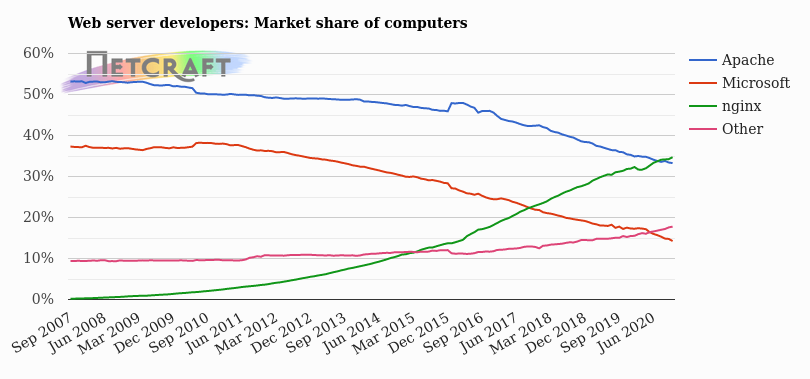
\includegraphics[width=0.95\textwidth]{img/NGINX.png}
    \caption{Anteil der Computer, auf denen NGINX eingesetzt wird~\cite{WebServerSurvey}}\label{fig:figure}
\end{figure}
\subsubsubsection{Installation von nginx}

\begin{lstlisting}[language=Bash, caption=Installation von NGINX,label={lst:nginxinstall}]
apt-get install nginx
\end{lstlisting}


\subsubsubsection{Installation von php und php-fpm}

PHP wird ebenfalls aus den Paketquellen installiert.
Außerdem wird das Modul php-fpm installiert, welches für nginx benötigt wird~\cite{InstallNginxPHP}.

\begin{lstlisting}[language=Bash, caption=PHP und PHP-FPM installation,label={lst:installphpphpfpm}]
> apt-get install php7.0 php7.0-fpm
\end{lstlisting}



\subsubsubsection{Installation von php-imagick über Paketquellen}

Zunächst wird versucht die PHP-Erweiterung für Imagemagick genauso über die Paketquellen zu installieren

\begin{lstlisting}[language=Bash, caption=Install PHP-Imagick Modul,label={lst:installphpmagick}]
> apt-get install php-imagick
\end{lstlisting}
\vspace{5mm}


Listet man sich nun alle installierten php module auf, wird ersichtlich, dass die Version die in den Paketquellen für Ubuntu 16.04 liegt nicht mit der installieten Version von Imagemagick kompatibel ist.
Dies lässt sich als positiv herausheben, da es zeigt, dass bei einer Neuinstallation von php7 und Imagemagick die Sicherheitslücke nicht mehr über php ausgenutzt werden kann.

\begin{lstlisting}[language=Bash, caption=PHP Module überprüfen,label={lst:checkmodule}]
> php -m | grep image
PHP Warning: Version warning: Imagick was compiled against Image Magick version 1673 but version 1682 is loaded. Imagick will run but may behave surprisingly in Unknown on line 0
\end{lstlisting}
\vspace{5mm}

Also muss das Package wieder deinstalliert werden und eine alte Version installiert werden.

\begin{lstlisting}[language=Bash, caption=Uninstall PHP-Imagick Modul,label={lst:uninstallimagick}]
> apt-get purge php-imagick
\end{lstlisting}
\vspace{5mm}

\newpage
\subsubsubsection{Installation von php-imagick from source}

Ältere Versionen von php-imagick können über PECL installiert werden.
PECL ist ein Package Repository für PHP Erweiterungen~\cite{PHPPecl}.

Bevor PECL genutzt werden kann, müssen noch einige Abhängigkeiten installiert werden~\cite{InstallPECLExtensions}.
\begin{lstlisting}[language=Bash, caption=Installiere PECL Abhängigkeiten,label={lst:installpecldeps}]
> apt-get install php-pear
> apt-get install php7.0-dev
> apt-get install pkg-config
\end{lstlisting}
\vspace{5mm}

Nun wird die Version 3.4.0 installiert:
\begin{lstlisting}[language=Bash, caption=PECL Install Imagick Modul,label={lst:peclinstallimagick}]
> pecl install imagick-3.4.0
\end{lstlisting}
\vspace{5mm}

Damit das imagick php modul in der CLI gefunden werden kann, muss es zunächst in der php.ini aktiviert werden.
Dafür wird ein neuer extension-Eintrag erstellt.

\begin{lstlisting}[language=Bash, caption=PHP Imagick aktivieren,label={lst:phpactivateimagick}]
> vim /etc/php/7.0/cli/php.ini
extension=imagick.so
\end{lstlisting}
\vspace{5mm}

\begin{lstlisting}[language=Bash, caption=PHP Überprüfe Imagick Modul,label={lst:phpcheckimagicksuccess}]
> php -m | grep imagick
imagick
\end{lstlisting}

\subsubsubsection{Konfiguration von NGINX}

Als erstes muss php in der site-config von nginx aktiviert werden. 
Die sock-Datei unter fastcgi\_pass muss existieren. 
Der Pfad ist bei anderen PHP Versionen unter Umstäden unterschiedlich. 
Um die Änderungen anzuwenden, muss nginx neu gestartet werden~\cite{InstallNginxPHP}.

\begin{lstlisting}[language=Bash, caption=NGINX Default-Config,label={lst:nginxdefaultconf}]
> vim /etc/nginx/sites-available/default
location ~ \.php$ {
    include snippets/fastcgi-php.conf;
    fastcgi_pass unix:/run/php/php7.0-fpm.sock;
}

> systemctl restart nginx
\end{lstlisting}
\vspace{5mm}

\newpage

\subsubsubsection{Aktivierung der des imagick Moduls für fpm}

Damit für nginx das imagick php modul ebenfalls aktiviert ist, muss die Erweiterung auch in der php.ini von fpm deklariert werden.

\begin{lstlisting}[language=Bash, caption=PHP-FPM Imagick Modul aktivieren,label={lst:phpfpmaddimagick}]
> vim /etc/php/7.0/fpm/php.ini
extension=imagick.so
\end{lstlisting}
\vspace{5mm}

Änderungen werden über ein Restart von fpm übernommen:
\begin{lstlisting}[language=Bash, caption=PHP-FPM Neustarten,label={lst:phpfpmrestart}]
service php7.0-fpm restart
\end{lstlisting}

\subsubsubsection{Überprüfen der Installation durch phpinfo()}

Um zu überprüfen, ob nun auf PHP Ebene Imagemagick gearbeitet werden kann, wird eine PHP Datei erstellt, in der die PHP Methode phpinfo() aufgerufen wird, welche zahlreiche Informationen zur Installierten PHP Umgebung anzeigt~\cite{PHPPhpinfoManual}.

\begin{lstlisting}[language=Bash, caption=info.php mit phpinfo(),label={lst:phpinfo}]
> vim /var/www/html/info.php

<?php
phpinfo();
?>
\end{lstlisting}
\vspace{5mm}

Ruft man nun die Seite über den Browser auf, sieht man auch das installierte imagick-Modul, sowie alle supporteten Datei-Formate.
Darunter auch einige Bild-Formate wie PNG, JPEG und MVG, welche für die Forum-Profil Seite benötigt werden.

\begin{figure}[H]
    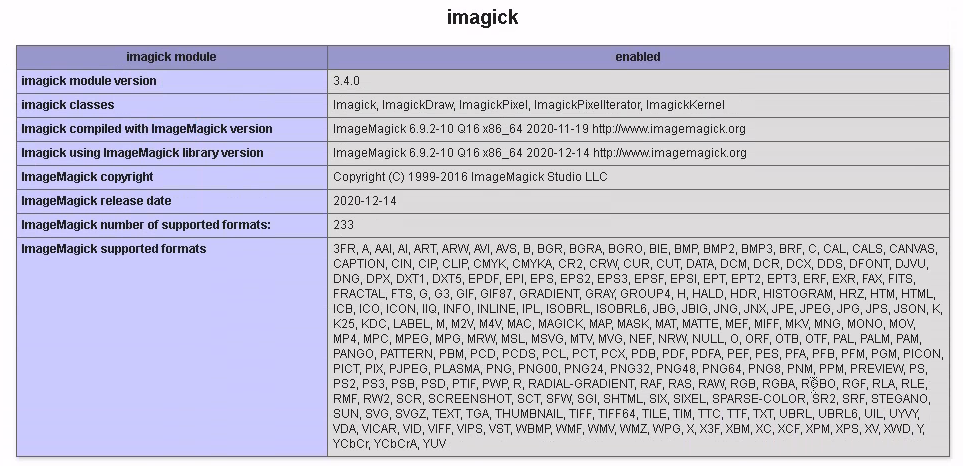
\includegraphics[width=1\textwidth]{img/phpinfo.png}
    \caption{imagick-Abschnitt aus phpinfo()}\label{fig:phpinfo}
\end{figure}

\subsubsubsection{Aufbau der PHP Website}

Als nächsten Schritt wird über HTML und CSS eine Profil-Seite aufgebaut, welche Links das Profilbild und einen Upload-Button zeigt.
Rechts sind noch einige weitere Informationen zu dem User zu finden.

\begin{figure}[H]
    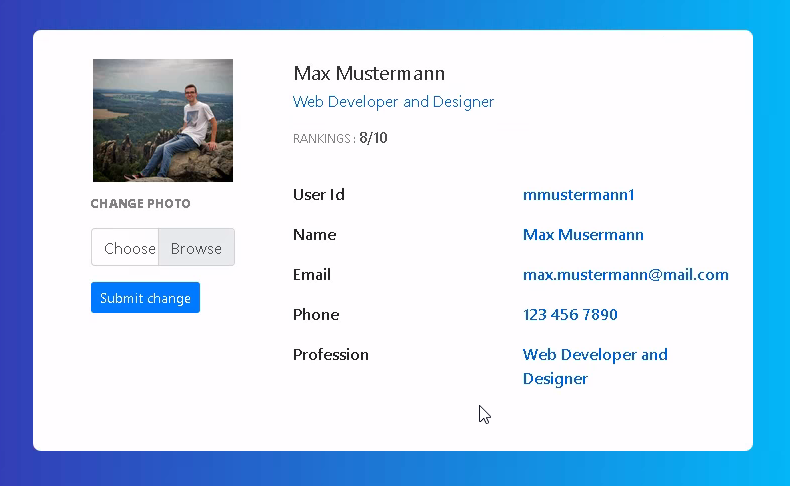
\includegraphics[width=1\textwidth]{img/ForumAufbau.png}
    \caption{Screenshot der Forum Profil-Seite}\label{fig:forumprofil}
\end{figure}
Für das Design wurde ein bestehendes Bootstrap Snippet genutzt, angepasst und um die Upload Funktionalität erweitert~\cite{BootSnapTemplate}.

Der relevante Imagemagick-Teil wird ausgeführt, sobald ein Bild in dem Filepicker ausgewählt und der Submit-Button betätigt wird.

\begin{lstlisting}[language=PHP, caption=Imagick skalieren und speichern,label={lst:imagickscalesave}]

<?php

if (isset($_POST['submit'])) {
  $dir = "uploads/";
  $file = $dir . basename($_FILES['file']['name']);
  echo move_uploaded_file($_FILES['file']['tmp_name'], $file);

  try {
	  $im = new Imagick($file);
	  $im->scaleImage(420, 240, true);
    $im->writeImage('profile.png');
  } catch (Exception $e) {
    echo $e->getMessage();
  }
}

?>
\end{lstlisting}
\vspace{5mm}

In diesem Fall wird das Bild in uploads/ abgelegt, per Imagemagick auf eine feste Größe skaliert~\cite{PHPImagickScaleImage} und anschließend nochmal in profile.png geschrieben.
Dei Datei unter dem Pfad profile.png wird in das Bild geladen.

\begin{lstlisting}[language=HTML, caption=Profile Image,label={lst:htmlimg}]
<div class="profile-img">
	<img src="profile.png" alt=""/>
</div>
\end{lstlisting}

